\documentclass[11pt,a4paper]{article}
\usepackage[margin=2.2cm]{geometry}
\usepackage{graphicx}
\usepackage{booktabs}
\usepackage{amsmath}
\usepackage{xcolor}
\usepackage[hidelinks]{hyperref}
\usepackage{caption}
\usepackage{float}
\captionsetup{font=small,labelfont=bf}
\setlength{\parskip}{0.45em}
\setlength{\parindent}{0pt}
\setlength{\emergencystretch}{2em}

\title{image denoising with bilateral filters:\\from a tuned classic filter to a neural-guided one}
\author{manas pandya\\[0.2em]\small nlp \& cv lab, task 07}
\date{october 2026}

\begin{document}
\maketitle

\begin{center}
\small
live demo: \url{https://nlp-cv-lab.vercel.app/p/bilateral-denoising}\\
code: \url{https://github.com/manasrpandya/NLP_CV_Lab/tree/main/projects/07-bilateral-denoising}\\
model: \url{https://huggingface.co/manasrpandya/bilateral-denoise-nbf}
\end{center}

\section{aim}

the task is to denoise images with bilateral filters. calling \texttt{cv2.bilateralFilter} once with
default-looking parameters does remove some noise, but it leaves two questions open: how good can the
bilateral filter get if its parameters are chosen properly, and how far is that from methods people actually
use for denoising. so the plan was a ladder of methods, each one a row in the results:

\begin{enumerate}
\itemsep0em
\item[(a)] the classic bilateral filter with $(d, \sigma_s, \sigma_r)$ grid-searched per noise level on held-out
images (an oracle, since it is told the true noise level),
\item[(b)] the same filter with blind parameters: estimate the noise level from the image and map it to
parameters with a fit from (a),
\item[(c)] iterated and joint (cross) bilateral filtering,
\item[(d)] a ``neural-guided bilateral'' filter (nbf), where a small cnn predicts $\sigma_s$, $\sigma_r$ and the
range guide for every pixel, trained end to end through a differentiable bilateral layer,
\item[(e)] reference points that are not bilateral: non-local means, BM3D and a pretrained DnCNN.
\end{enumerate}

everything is evaluated with PSNR/SSIM on standard test sets at three noise levels plus one real-noise set,
and the nbf model is exported to ONNX and runs in the browser on the demo page, next to a webgl version of
the classic filter that runs in real time on a webcam.

\section{background}

the bilateral filter \cite{tomasi98} replaces each pixel $p$ by a normalised weighted average of its
neighbours $q$ in a window $\Omega_p$:
\begin{equation}
\hat{x}_p = \frac{\sum_{q\in\Omega_p} w_{pq}\, y_q}{\sum_{q\in\Omega_p} w_{pq}}, \qquad
w_{pq} = \exp\!\Big(-\frac{\|p-q\|^2}{2\sigma_s^2}\Big)\exp\!\Big(-\frac{(g_p-g_q)^2}{2\sigma_r^2}\Big),
\label{eq:bf}
\end{equation}
where $y$ is the noisy image and $g$ is the image used for the range term. for the plain filter $g=y$; for
the joint or cross bilateral filter $g$ is a different (here: smoothed) image. the spatial term makes it a
blur, the range term stops it from averaging across edges. the problem is that with $g=y$ the range term
sees the noise too: if $\sigma_r$ is small compared to the noise, noisy pixels only average with themselves,
and if it is large, the filter turns into a gaussian blur and edges go. there is one global $(\sigma_s,
\sigma_r)$ for the whole image, which is a poor fit for images with both flat areas and texture.

this has been attacked in several ways. the adaptive bilateral filter of gavaskar and chaudhury
\cite{gavaskar19} lets the range kernel centre and width change per pixel. hdrnet \cite{gharbi17} predicts
the coefficients of a bilateral grid with a cnn, and bilateral neural networks \cite{jampani16} learn the
filter itself in a permutohedral lattice. my nbf model sits closest to the adaptive filter: the output is
still eq.~\ref{eq:bf}, only $\sigma_s$, $\sigma_r$ and $g$ are predicted per pixel by a network. the
reference methods are non-local means \cite{buades05}, BM3D \cite{dabov07} and DnCNN \cite{zhang17}.

\section{data}

\textbf{training.} the 400 BSD images (180$\times$180, gray) used by DnCNN \cite{zhang17}. the last 32 are
held out as a validation set and are used for every parameter search and for model selection, so the test
sets are never touched for tuning. DIV2K was not added, BSD400 was enough for a model this small.

\textbf{testing.} Set12, BSD68 and Kodak24 (converted to gray), with additive gaussian noise at
$\sigma\in\{15,25,50\}$ (on the 0-255 scale). noise is drawn once with a fixed seed per image and
$\sigma$, and is not clipped, which is the usual convention. as a real-noise test i used 320 of the 1280
SIDD validation crops \cite{sidd18} (every 4th, so all 40 scenes are covered, 256$\times$256, converted to
gray), taken from a copy on the hugging face hub. the download script \texttt{bden.data} fetches and
caches all of it.

\section{method}

\subsection{(a) tuned bilateral}

grid search of \texttt{cv2.bilateralFilter} over $d\in\{3,\dots,11\}$, $\sigma_s\in[0.8,5]$ and
$\sigma_r\in[0.8,6]\cdot\sigma$, at $\sigma=5,10,\dots,60$ on the 32 validation images, maximising mean
PSNR. many window sizes tie once the spatial gaussian has decayed, so i keep the smallest $d$ within 0.02 dB
of the best. the result (table in \texttt{results/auto\_fit.json}) is quite regular: $\sigma_s$ grows
slowly from 0.8 to 2 px, and the best $\sigma_r$ is $2.5\sigma$ at low noise but climbs to $4\sigma$ at
$\sigma=60$, which fits a line $\sigma_r\approx 4.17\sigma-28.8$. at high noise the best filter is
basically a gaussian blur with a mild edge stop, which already says a lot about the limits of the plain
bilateral filter.

\subsection{(b) blind auto parameters}

the noise level is estimated from the noisy image with immerkaer's method \cite{immerkaer96} (mean
absolute response of a laplacian-difference mask) and, for comparison, the wavelet estimate
$\mathrm{median}(|HH|)/0.6745$ \cite{donoho94}. both are biased upwards by image texture, so each gets a
linear calibration $\hat\sigma = a\,\sigma_{raw}+b$ fitted on the validation images. the calibrated
estimate is mapped to $(d,\sigma_s,\sigma_r)$ by linear interpolation in the table from (a). the same
estimator and table are implemented in javascript for the demo's auto mode.

\subsection{(c) iterated and joint bilateral}

the iterated filter runs the bilateral filter $n$ times with a smaller $\sigma_r$; the joint filter uses
$g=G_{\sigma_g} * y$, a lightly gaussian-smoothed copy of the noisy image, for the range term so that it
is less fooled by the noise. both were tuned on the validation set ($n$, $\sigma_s$, $\sigma_r$, $\sigma_g$)
at $\sigma\in\{5,10,15,25,50\}$ and interpolated in between. two iterations always won. the joint
filter used my pytorch bilateral layer (below), which matches cv2 to within $5\cdot10^{-3}$ (unit test).

\subsection{(d) neural-guided bilateral (nbf)}

\textbf{bilateral layer.} eq.~\ref{eq:bf} written in pytorch with a $k\times k$ disc window ($k=7$,
37 taps, reflect padding, like cv2). $\sigma_s$ and $\sigma_r$ can be scalars or per-pixel maps, and
there is an optional guide. the weights are computed in the log domain and normalised with a softmax over
the taps, which is the same as eq.~\ref{eq:bf} but does not underflow for tiny $\sigma_r$. the plan said
``unfold-based''; i ended up stacking 37 shifted slices of the padded image instead of
\texttt{F.unfold}, because that exports to plain \texttt{Slice}/\texttt{Concat} ONNX ops which every
runtime supports (including onnxruntime-web on webgpu), and it costs the same memory.

\textbf{network.} a small 3-level unet (16/32/48 channels, leaky relu, strided conv down, bilinear up,
92.7k parameters) takes the noisy image and outputs 5 maps: $\sigma_s$ and $\sigma_r$ for two bilateral
passes and a guide residual. they go through bounded activations,
$\sigma_s = 0.3 + 3.2\,\mathrm{sigmoid}(\cdot)$ px and $\sigma_r = 0.003+0.5\,\mathrm{sigmoid}(\cdot-2)$.
pass 1 filters the noisy image with range weights from the guide $g=y+r$; pass 2 filters the result of
pass 1 with itself as guide. so the output is always a convex combination of noisy pixels in a 13$\times$13
neighbourhood, it can't invent structure that is not there, which a plain cnn can.

\textbf{training.} random 80$\times$80 crops with flips and rotations, batch 32, gaussian noise with
$\sigma\sim U(0,55)$ per crop, so one model is blind to the noise level. L1 loss, AdamW with lr
$2\cdot10^{-3}$, cosine decay over 9000 iterations, gradient clipping at 1. this takes 7.5-15 minutes on the
laptop gpu (rtx 2050, the spread is cpu contention from evaluation runs going on at the same time, the
iteration budget is fixed so the runs are comparable). the checkpoint with the best validation PSNR at
$\sigma=25$ is kept. the four models trained (nbf and three ablations) used about 45 minutes of gpu time
in total.

\textbf{export.} the model is exported to ONNX (opset 17, dynamic batch and size) with both the image and
the 5 maps as outputs. the file is 462 kB and the max abs difference to pytorch on three test images is
$7.6\cdot10^{-6}$ (checked with the shared \texttt{labcore.parity} helper, and in a unit test).

\subsection{(e) references}

cv2 \texttt{fastNlMeansDenoising} with $h$ tuned per $\sigma$ on validation, the \texttt{bm3d} package
with the true $\sigma$, and the blind gray DnCNN-B weights from the KAIR model zoo \cite{zhang17}
(666k parameters, trained on the same BSD400 images with $\sigma\in[0,55]$, so a fair blind
comparison). on SIDD every method that needs a noise level gets the immerkaer estimate.

\section{experiments and results}

\begin{table}[H]
\centering
\small
\setlength{\tabcolsep}{2.6pt}
\begin{tabular}{llcccccccccc}
\toprule
 & & \multicolumn{3}{c}{Set12} & \multicolumn{3}{c}{BSD68} & \multicolumn{3}{c}{Kodak24} & SIDD \\
\cmidrule(lr){3-5}\cmidrule(lr){6-8}\cmidrule(lr){9-11}\cmidrule(lr){12-12}
 & Method & 15 & 25 & 50 & 15 & 25 & 50 & 15 & 25 & 50 & real \\
\midrule
- & Noisy input & 24.69 & 20.32 & 14.76 & 24.79 & 20.48 & 14.91 & 24.74 & 20.39 & 14.78 & 27.02 \\
a & Bilateral, tuned per sigma & 30.35 & 27.44 & 24.03 & 29.71 & 26.96 & 23.98 & 30.38 & 27.54 & 24.57 & 30.47 \\
b & Bilateral, blind auto params & 30.29 & 27.39 & 24.03 & 29.60 & 26.90 & 23.97 & 30.31 & 27.48 & 24.56 & 30.47 \\
c & Iterated bilateral & 30.45 & 27.82 & 24.57 & 29.81 & 27.20 & 24.36 & 30.62 & 28.00 & 24.97 & \textbf{30.83} \\
c & Joint bilateral (smoothed guide) & 30.88 & 28.17 & 24.35 & 30.00 & 27.45 & 24.05 & 30.81 & 28.15 & 24.54 & 30.75 \\
d & Neural-guided bilateral (ours) & \textbf{31.93} & \textbf{29.60} & \textbf{26.44} & \textbf{30.82} & \textbf{28.38} & \textbf{25.48} & \textbf{32.11} & \textbf{29.79} & \textbf{26.84} & 27.27 \\
\midrule
e & Non-local means (cv2) & 30.36 & 27.82 & 24.28 & 29.37 & 26.68 & 23.69 & 30.37 & 27.65 & 24.61 & 32.59 \\
e & BM3D & 32.40 & 30.00 & 26.73 & 31.15 & 28.63 & 25.71 & 32.37 & 29.96 & 27.02 & 28.21 \\
e & DnCNN-B (pretrained) & 32.68 & 30.36 & 27.18 & 31.62 & 29.16 & 26.23 & 32.78 & 30.42 & 27.51 & 27.48 \\
\bottomrule
\end{tabular}

\caption{PSNR (dB). bold is the best bilateral variant per column. (a) and (c) are told the true $\sigma$
on the synthetic sets, (b), (d) and DnCNN are blind.}
\label{tab:main}
\end{table}

table~\ref{tab:main} is the main result. a properly tuned bilateral filter gives about +6.5 dB at
$\sigma=25$ (26.96 dB on BSD68), and the blind version (b) loses about 0.1 dB of that, so the
estimator plus lookup table is good enough to replace manual tuning. iterated and joint filtering add
0.2-0.6 dB, the joint filter is better at low noise and the iterated one at $\sigma=50$. the nbf model is
a clear step up, +1.4 dB over (a) on BSD68 at $\sigma=25$ and +1.5 dB at $\sigma=50$, it beats NLM
everywhere on the synthetic sets and ends up 0.2-0.5 dB below BM3D (which is told the true noise level).
DnCNN-B, with about 7 times the parameters and no bilateral constraint, is still 0.7-0.8 dB better.

\begin{figure}[H]
\centering
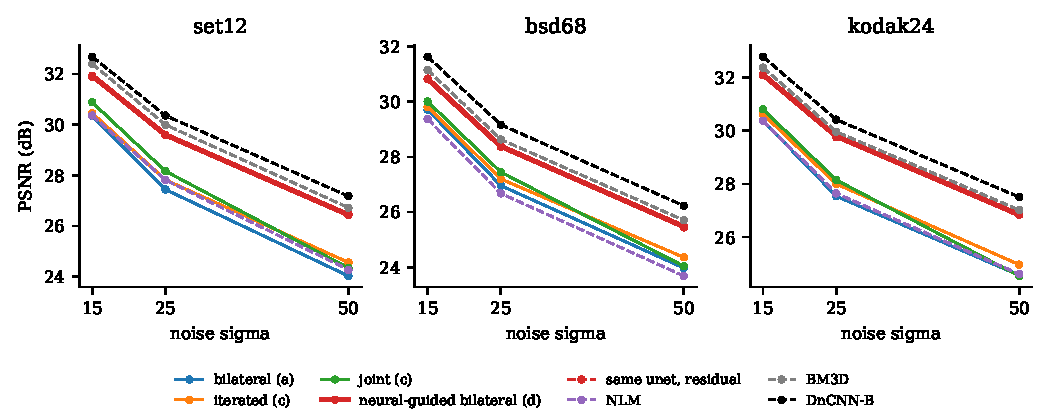
\includegraphics[width=\linewidth]{figs/psnr_sigma.pdf}
\caption{PSNR against the noise level on the three test sets.}
\label{fig:psnr}
\end{figure}

\begin{figure}[H]
\centering
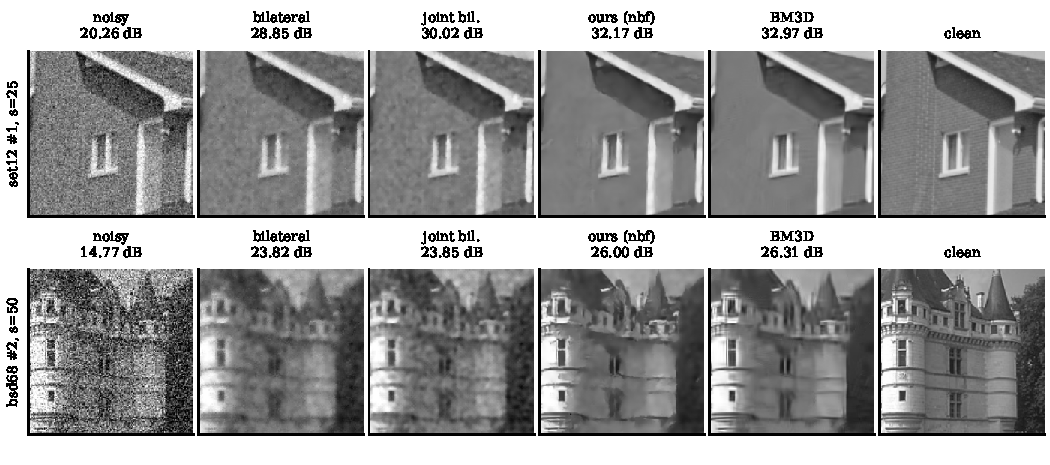
\includegraphics[width=\linewidth]{figs/crops.pdf}
\caption{crops, PSNR of the whole image underneath. the plain bilateral filter leaves blotchy noise in flat
areas at $\sigma=25$ and blurs everything at $\sigma=50$.}
\label{fig:crops}
\end{figure}

\textbf{ssim} follows the same order (table~\ref{tab:ssim}), the gap between plain bilateral and the rest
is larger in SSIM than in PSNR, because the leftover noise in flat areas is exactly what SSIM punishes.

\begin{table}[H]
\centering
\small
\begin{tabular}{lcccc}
\toprule
method & 15 & 25 & 50 & SIDD \\
\midrule
noisy input & 0.590 & 0.416 & 0.218 & 0.432 \\
bilateral, tuned per sigma & 0.820 & 0.711 & 0.570 & 0.600 \\
bilateral, blind auto params & 0.815 & 0.705 & 0.569 & 0.600 \\
iterated bilateral & 0.836 & 0.744 & 0.596 & 0.615 \\
joint bilateral (smoothed guide) & 0.836 & 0.740 & 0.559 & 0.612 \\
neural-guided bilateral (ours) & 0.877 & 0.807 & 0.682 & 0.444 \\
non-local means (cv2) & 0.826 & 0.722 & 0.579 & 0.666 \\
BM3D & 0.880 & 0.809 & 0.691 & 0.491 \\
DnCNN-B (pretrained) & 0.892 & 0.830 & 0.719 & 0.453 \\
\bottomrule
\end{tabular}

\caption{SSIM on BSD68 and SIDD.}
\label{tab:ssim}
\end{table}

\textbf{method noise.} fig.~\ref{fig:mnoise} shows $y-\hat x$ for one image. ideally this is pure noise.
the plain bilateral filter clearly removes edges (the roof line and the window frames show up), the joint
filter a bit less, while the method noise of nbf and BM3D looks like plain noise.

\begin{figure}[H]
\centering
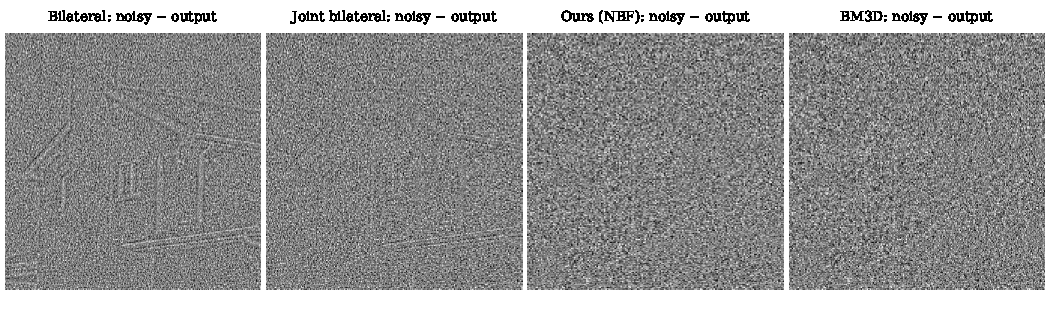
\includegraphics[width=\linewidth]{figs/method_noise.pdf}
\caption{method noise (noisy minus output) on Set12 house, $\sigma=25$. visible structure means detail
that the filter removed.}
\label{fig:mnoise}
\end{figure}

\subsection{what the network learned}

fig.~\ref{fig:maps} shows the predicted maps for the first pass. $\sigma_r$ is low on edges and in
texture (the tripod, the coat, the grass) and high in flat regions like the sky, which is the adaptive
behaviour i hoped for. $\sigma_s$ is small along edges and large in flat areas, and the whole map shifts
up when the noise goes up. the guide turned out to be interesting: it is not in image units at all, its
values go up to about 4, i.e. the network scales the guide up by about 4$\times$. since only $(g_p-g_q)/\sigma_r$
matters this is the same as using a $\sigma_r$ four times smaller, and it seems the network did this to get
around my upper bound on $\sigma_r$ for pass 1, which most pixels sit close to. that bound was a design
mistake but a harmless one.

\begin{figure}[H]
\centering
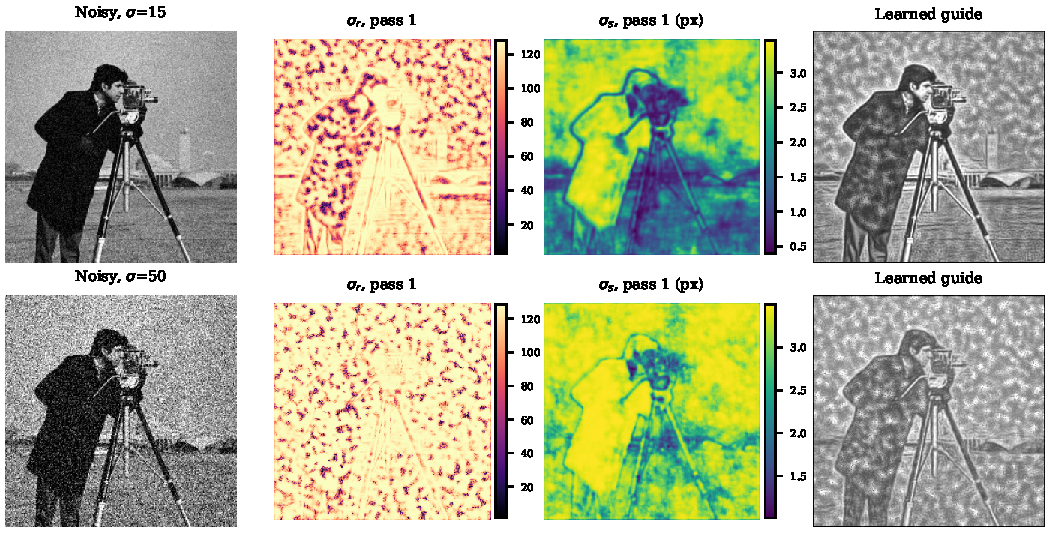
\includegraphics[width=\linewidth]{figs/maps.pdf}
\caption{nbf maps for pass 1 on Set12 cameraman at $\sigma=15$ (top) and 50 (bottom). $\sigma_r$ on the
0-255 scale, $\sigma_s$ in pixels.}
\label{fig:maps}
\end{figure}

fig.~\ref{fig:params} averages the maps over 20 BSD68 images at many noise levels. the model never sees
$\sigma$, but the median pass-1 $\sigma_s$ goes from 0.3 px at $\sigma=0$ to 3 px at $\sigma=60$, and the
pass-2 $\sigma_r$ grows almost linearly with $\sigma$, much like the grid search optimum for the classic
filter but about 4-5 times smaller. so pass 2 behaves like a classic bilateral filter cleaning up after
pass 1, with $\sigma_s$ pinned at the 3.5 px maximum (with a 7$\times$7 window that is close to a disc box
filter). at $\sigma=0$ the model shrinks pass 1 to almost nothing, so it doesn't damage clean images.

\begin{figure}[H]
\centering
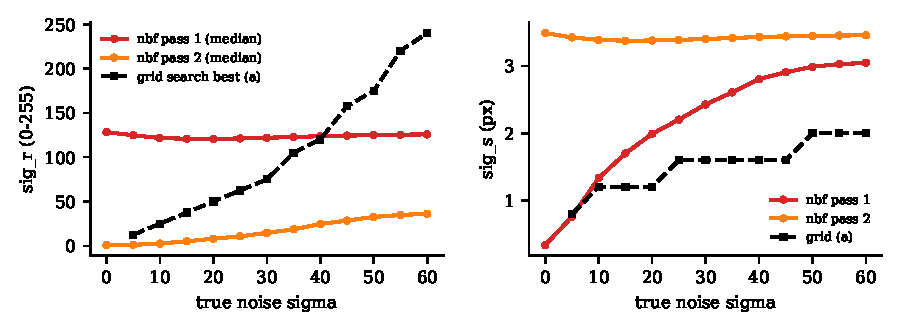
\includegraphics[width=0.8\linewidth]{figs/params_sigma.pdf}
\caption{median predicted $\sigma_r$ and $\sigma_s$ against the true noise level, compared with the
grid-search optimum of the classic filter (a).}
\label{fig:params}
\end{figure}

\subsection{ablations}

all variants were trained with the same budget (9000 iterations, same seed and data order).

\begin{table}[H]
\centering
\small
\begin{tabular}{lrcccc}
\toprule
Variant & Params & Val (25) & BSD68 15 & 25 & 50 \\
\midrule
Neural-guided bilateral (ours) & 92.7k & 29.14 & 30.82 & 28.38 & 25.48 \\
NBF, no guide & 92.7k & 28.72 & 30.76 & 28.28 & 25.27 \\
NBF, one pass & 92.6k & 29.02 & 30.86 & 28.35 & 25.19 \\
Same U-Net, plain residual & 92.6k & 29.17 & 30.83 & 28.36 & 25.45 \\
\bottomrule
\end{tabular}

\caption{ablations. ``same unet, plain residual'' is the same network predicting the noise directly,
without any bilateral structure.}
\label{tab:abl}
\end{table}

the learned guide is the most useful part: without it (pass 1 uses the noisy image for the range
weights, like the plain filter) validation PSNR drops by 0.4 dB, on BSD68 the drop is smaller, 0.06 dB at
$\sigma=15$ growing to 0.21 dB at $\sigma=50$. the second pass only matters at high noise: with one pass
the model is as good or slightly better at $\sigma\le25$ but loses 0.29 dB at $\sigma=50$, where a single
7$\times$7 window is simply too small.

the honest comparison is the last row. the same unet trained to predict the noise directly, without any
bilateral structure, is just as good: 0.03 dB better on validation and within 0.03 dB on BSD68. so the
bilateral constraint does not cost PSNR, but it doesn't buy any either. what it does give is an output
that is always a weighted average of nearby noisy pixels (so it can't hallucinate texture), parameter
maps that can be looked at and explained (fig.~\ref{fig:maps}), and a model that reduces to almost
identity on clean input. the price is runtime, the two bilateral passes roughly double the cost of the
unet (table~\ref{tab:bench}). the one place the structure does help is early training (fig.~\ref{fig:curves}):
after 1000 iterations nbf is 0.5 dB ahead of the plain unet, which only catches up after about 4000.
with a shorter budget or less data the bilateral prior would probably matter more.

\begin{figure}[H]
\centering
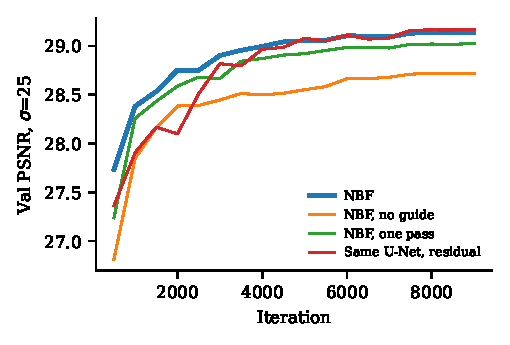
\includegraphics[width=0.48\linewidth]{figs/curves.pdf}
\caption{validation PSNR at $\sigma=25$ during training.}
\label{fig:curves}
\end{figure}

\subsection{noise estimation}

\begin{table}[H]
\centering
\small
\begin{tabular}{lccc}
\toprule
Estimator & 15 & 25 & 50 \\
\midrule
Immerkaer & 0.81 (-0.34) & 0.67 (-0.43) & 0.29 (-0.08) \\
Wavelet & 0.95 (-0.29) & 0.84 (-0.41) & 0.54 (-0.24) \\
\bottomrule
\end{tabular}

\caption{mean absolute error (and bias) of the calibrated noise estimators on all synthetic test images.}
\label{tab:est}
\end{table}

after calibration both estimators are within about 1 grey level of the true $\sigma$ on gaussian noise
(table~\ref{tab:est}, fig.~\ref{fig:est}); immerkaer is a bit better and much cheaper, so it is the one
used for (b) and in the browser. on SIDD it is a different story, see below.

\begin{figure}[H]
\centering
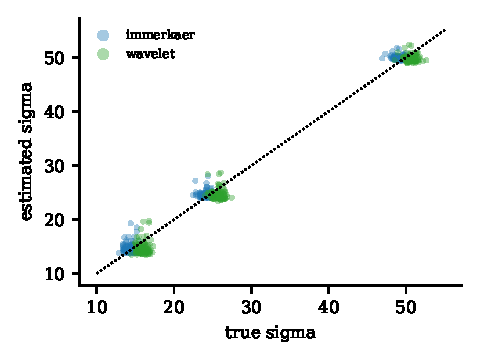
\includegraphics[width=0.45\linewidth]{figs/estimator.pdf}
\caption{calibrated estimate against the true $\sigma$ on all synthetic test images.}
\label{fig:est}
\end{figure}

\subsection{runtime}

\begin{table}[H]
\centering
\small
\begin{tabular}{lrrr}
\toprule
method & cpu (ms) & gpu (ms) & params \\
\midrule
bilateral, tuned per sigma & 12 & - & - \\
iterated bilateral & 14 & - & - \\
joint bilateral (smoothed guide) & 71 & - & - \\
non-local means (cv2) & 162 & - & - \\
BM3D & 5040 & - & - \\
neural-guided bilateral (ours) & 291$^*$ & 27.5 & 93k \\
same unet, plain residual & 154$^*$ & 13.1 & 93k \\
DnCNN-B (pretrained) & 2506$^*$ & 134.4 & 666k \\
nbf, onnx runtime & 501$^*$ & - & - \\
\bottomrule
\end{tabular}

\caption{time for one 512$\times$512 gray image, median of 5 runs. cpu is one thread, $^*$ means 4 threads.
gpu is the rtx 2050. the machine was not idle (another job was running), so treat these as rough.}
\label{tab:bench}
\end{table}

the plain bilateral filter is by far the cheapest (table~\ref{tab:bench}), and in the browser the webgl
shader runs it in real time on a 640$\times$480 webcam stream. nbf is about 5 times faster than DnCNN on the gpu and 9 times on
cpu. about half of its gpu time is the two bilateral passes (the plain unet alone takes 13 ms), the 37
shifted copies per pass are memory bound rather than compute bound.

\section{discussion and limitations}

\textbf{where bilateral filtering loses.} even tuned perfectly, the plain bilateral filter is 1.7 dB
behind BM3D at $\sigma=25$ and 2.2 dB behind DnCNN. it only looks at a small window and its range test is
done on noisy values, so at high noise it has to choose between leaving noise and blurring, and the
grid search says blurring wins (best $\sigma_r$ is 4$\sigma$). the iterated and joint versions help a
little, they don't change the picture.

\textbf{real noise.} on SIDD the ranking flips. the gaussian-trained networks barely change the image
(nbf +0.25 dB, DnCNN +0.5 dB), while the classical filters driven by the immerkaer estimate gain 3.5 dB
and NLM 5.6 dB. real smartphone noise after the camera pipeline is spatially correlated and signal
dependent; the residual between noisy and clean SIDD crops has a median standard deviation of 9.9 grey
levels, but immerkaer estimates 4.2 because most of the noise energy is at lower frequencies than the
laplacian mask looks at. the networks were trained on white noise, see little high-frequency noise, and
treat the rest as texture. the classical filters still smooth because they are told some noise is
present. training nbf on realistic noise (e.g. SIDD medium training pairs or a simple
correlated-noise model) would be the obvious next step and was out of the time budget here.

\textbf{color.} everything was evaluated on gray images. in the demo the filters run per channel on
rgb, which works but leaves some chroma noise, a joint color range kernel would be better.

\textbf{browser.} the browser runs nbf on 256$\times$256 tiles with 24 px of context on each side to keep
memory low on phones. on the wasm fallback a 768$\times$512 rgb image took about 5 s on my (busy) laptop;
webgpu is faster where it works, and the worker falls back to wasm if a webgpu warm-up run fails or hangs
(which happened with a software adapter in headless chrome).

\section{how to run}

\begin{verbatim}
cd projects/07-bilateral-denoising
uv sync --extra ref
uv run python -m bden.data          # data + dncnn weights into data/
uv run python -m bden.search        # (a)/(b) grid search + estimator calibration
uv run python -m bden.tune          # (c) and nlm params
uv run python -m bden.train --mdl nbf
uv run python -m bden.evaluate --methods noisy bf_oracle bf_auto bf_iter \
    bf_joint nlm bm3d nbf dncnn
uv run python -m bden.export && uv run python -m bden.bench
uv run python -m bden.figs && uv run python -m bden.tables
uv run pytest -q
\end{verbatim}

the demo page source is in \texttt{web/app/p/bilateral-denoising} and
\texttt{web/lib/bilateral-denoising} of the same repo.

\begin{thebibliography}{99}
\small
\bibitem{tomasi98} c. tomasi and r. manduchi. bilateral filtering for gray and color images. iccv 1998.
\bibitem{gavaskar19} r. g. gavaskar and k. n. chaudhury. fast adaptive bilateral filtering. ieee tip 28(2), 2019.
\bibitem{gharbi17} m. gharbi, j. chen, j. t. barron, s. w. hasinoff and f. durand. deep bilateral learning for
real-time image enhancement. siggraph 2017.
\bibitem{jampani16} v. jampani, m. kiefel and p. v. gehler. learning sparse high dimensional filters: image
filtering, dense crfs and bilateral neural networks. cvpr 2016.
\bibitem{buades05} a. buades, b. coll and j.-m. morel. a non-local algorithm for image denoising. cvpr 2005.
\bibitem{dabov07} k. dabov, a. foi, v. katkovnik and k. egiazarian. image denoising by sparse 3-d
transform-domain collaborative filtering. ieee tip 16(8), 2007.
\bibitem{zhang17} k. zhang, w. zuo, y. chen, d. meng and l. zhang. beyond a gaussian denoiser: residual
learning of deep cnn for image denoising. ieee tip 26(7), 2017.
\bibitem{immerkaer96} j. immerk\ae r. fast noise variance estimation. cviu 64(2), 1996.
\bibitem{donoho94} d. l. donoho and i. m. johnstone. ideal spatial adaptation by wavelet shrinkage.
biometrika 81(3), 1994.
\bibitem{sidd18} a. abdelhamed, s. lin and m. s. brown. a high-quality denoising dataset for smartphone
cameras. cvpr 2018.
\end{thebibliography}

\end{document}
